\chapter{Ecuación de onda}
\label{cap:wave}
\begin{resumen}
		En este capítulo presentamos la ecuación de onda en una y dos dimensiones espaciales.
	En cada caso formulamos primero el problema de valores iniciales y de contorno, y damos condiciones de existencia y unicidad de la solución. Tras ello, introduciremos discretizaciones en diferencias finitas y detallaremos los algoritmos resultantes.
\end{resumen}

\section{Caso lineal}
La ecuación de onda tiene la forma
\begin{equation}
	\frac{\partial^2u}{\partial t^2} - c^2\frac{\partial^2u}{\partial x^2} = 0
\end{equation}
y consideraremos el dominio $R=\{(x,t) \hspace{5px} | \hspace{5px} 0\leq t\}$ y el problema inicial que fija el valor de la función y su derivada en $t=0$, lo que nos deja con el problema 
\begin{equation}
	\label{eq:1dwave}
\begin{cases}
	\frac{\partial^2u}{\partial t^2}(x,t) - c^2\frac{\partial^2u}{\partial x^2}(x,t) = 0, & -\infty < x < \infty, \hspace{5px} 0\leq t,\\
	u(x,0) = f(x), & -\infty < x < \infty, \\
	\frac{\partial u(x,0)}{\partial t} = g(x), & -\infty < x < \infty.
\end{cases}
\end{equation}
\subsection{Existencia y unicidad}
Como es costumbre, empezamos con un resultado\footnote{Este puede encontrarse en \cite{1dwavedem}} sobre la existencia y unicidad de la solución. Supongamos que $u$ fuera solución de \eqref{eq:1dwave}, si hacemos el cambio de variable $\xi = x-ct, \hspace{5px} \eta = x+ct$, aplicando la regla de la cadena, obtenemos
\begin{equation}
	\frac{\partial u}{\partial x} = \frac{\partial\xi}{\partial x}\frac{\partial u}{\partial\xi} + \frac{\partial\eta}{\partial x}\frac{\partial u}{\partial\eta} = \frac{\partial u}{\partial\xi} + \frac{\partial u}{\partial\eta}
\end{equation}
y
\begin{equation}
	\frac{\partial u}{\partial t} = \frac{\partial\xi}{\partial t}\frac{\partial u}{\partial\xi} + \frac{\partial\eta}{\partial t}\frac{\partial u}{\partial\eta} = -c\frac{\partial u}{\partial\xi} +c \frac{\partial u}{\partial\eta}.
\end{equation}
Derivando una segunda vez, llegamos a
\begin{equation}
	\frac{\partial^2u}{\partial x^2} = \frac{\partial^2u}{\partial \xi^2}+2\frac{\partial^2u}{\partial\xi\partial\eta}+\frac{\partial^2u}{\partial\eta^2}
\end{equation}
y
\begin{equation}
	\frac{\partial^2u}{\partial t^2} = c^2\frac{\partial^2u}{\partial \xi^2}-2c^2\frac{\partial^2u}{\partial\xi\partial\eta}+c^2\frac{\partial^2u}{\partial\eta^2}.
\end{equation}
Luego, si sustituimos en \eqref{eq:1dwave} utilizando las últimas expresiones, concluimos que $u$ tiene que cumplir la siguiente ecuación
\begin{equation}
	\frac{\partial^2 u}{\partial\xi\partial\eta} = 0.
\end{equation}
Si integramos dos veces, podemos observar que $u$ tiene que ser de la forma
\begin{equation}
	\label{eq:1dwave2}
	u(x,t) = P(\xi) + Q(\eta) = P(x-ct) + Q(x+ct)
\end{equation}
para unas funciones $P$ y $Q$ arbitrarias, como $u$ es solución de \eqref{eq:1dwave}, tiene que cumplir sus restriccioines, por lo que $P$ y $Q$ tienen que cumplir.
\begin{equation}
	P(x) + Q(x) = f(x), \hspace{20px} P'(x) - Q'(x) = \frac{1}{c}g(x). 
\end{equation}
Ahora, si integramos la segunda relación en el intervalo $[0,x]$, y la sumamos y restamos a la primera, concluimos que las funciones $P$ y $Q$ tienen que ser exactamente de la forma (suponiendo que la función $g$ sea integrable)
\begin{equation}
	P(x) = \frac{1}{2}f(x) + \frac{1}{2c}\int_{0}^{x}g(\zeta)d\zeta + K
\end{equation}
y
\begin{equation}
	Q(x) = \frac{1}{2}f(x) - \frac{1}{2c}\int_{0}^{x}g(\zeta)d\zeta - K,
\end{equation}
siendo $K=\frac{1}{2}[P(0)-Q(0)]$.

Por tanto, si suponemos que \eqref{eq:1dwave} tiene solución, hemos encontrado como tienen que ser las funciones $P$ y $Q$, pero si ahora sustituimos eso en \eqref{eq:1dwave2}, concluimos que la solución tiene que ser exactamente de la forma
\begin{equation}
	\label{eq:1dwavesol}
	u(x,t) = \frac{1}{2}[f(x+ct)+f(x-ct)] + \frac{1}{2c}\int_{x-ct}^{x+ct}g(\zeta)d\zeta.
\end{equation}

Con esto no solo hemos probado que la solución es única (ya que cualquier solución arbitraria tiene que ser exactamente la función \eqref{eq:1dwavesol}), también hemos probado que siempre que la función $u$ esté bien definida (osea, siempre que $g$ sea integrable), existe una solución a la ecuación, por tanto tenemos el siguiente resultado.

\begin{teorema}[Existencia y unicidad]
	Si $g$ es una función integrable, el problema \eqref{eq:1dwave} tiene una única solución.
\end{teorema}



\subsection[Aproximación de la solución]{Aproximación de la solución\footnote{Las demostraciones de toda esta sección son modificaciones propias de \cite{anummeth}}}

Teniendo en cuenta toda la notación descrita en la Sección \ref{sec:notacion}, así como la definición \ref{def:malla2d}, vamos a aproximar la solución por la función $U$ en los puntos de la malla $M^2(a,b,0,T,n_x,n_t)$, que a partir de ahora denotaremos simplemente como $M$. Como en este caso el dominio es el semiplano $\{0\leq t\}$, está claro que $(x_i,t_j)\in R\iff 0\leq j$.

Pediremos a la función de aproximación $U$ que cumpla la igualdad $\frac{\partial^2u}{\partial t^2} = c^2\frac{\partial^2u}{\partial x^2}$, pero sustituyendo las derivadas parciales por sus aproximaciones mediante las diferencias finitas \eqref{eq:not_second}, lo que nos lleva a lo siguiente
\begin{multline}
	U^{t\bar t}(x,t) - c^2U^{x\bar{x}}(x,t) = 0 \Rightarrow \frac{1}{\Delta t^2}[U(x,t + \Delta t)-2U(x,t)+u(x, t - \Delta t)]  = \\ \left(\frac{c}{\Delta x}\right)^2[U(x+\Delta x,t)-2U(x,t)+U(x-\Delta x, t)].
\end{multline}
Sean $i$ y $j$ tales que $x=x_i$ y $t=t_j$, si reescribimos la ecuación anterior, obtenemos
\begin{equation}
	\begin{split}
	\frac{1}{\Delta t^2}[U_{i,j+1}-2U_{i,j}+U_{i,j-1}] = \left(\frac{c}{\Delta x}\right)^2[U_{i+1,j}-2_{i,j}+U_{i-1,j}] \Rightarrow \\
	U_{i,j+1} = \left(c\frac{\Delta t}{\Delta x}\right)^2[U_{i+1,j}-2U_{i,j}+U_{i-1,j}] + 2U_{i,j} - U_{i,j-1}	
	\end{split}
\end{equation}
que, tras combinar elementos y definir $\lambda=c\frac{\Delta t}{\Delta x}$, nos lleva a la fórmula explícita
\begin{equation}
	\label{eq:1dwave_formula}
	U_{i,j+1} =  2\left[1 - \lambda^2\right]U_{i,j} + \lambda^2[U_{i+1,j} + U_{i-1,j}] - U_{i,j-1}, \hspace{5px} j\geq1.
\end{equation}

La fórmula \eqref{eq:1dwave_formula} nos permite calcular el valor de $U_{i,j}$ para cualquier $i\in\mathbb{Z}$ siempre que conozcamos los valores de $U_{i,j-1}$ y $U_{i,j-2} \forall i\in\mathbb{Z}$, luego antes de poder utilizar esta fórmula, necesitaremos aproximar los valores de $U_{i,0}$ y $U_{i,1}$.

Los valores para $t=0$ son sencillos, pues por las condiciones iniciales sabemos el valor exacto de la función $u$ en estos puntos, por lo que definimos $U_{i,0}:=f(a+i\Delta x)\hspace{5px} \forall i\in\mathbb{Z}$ y sabemos que el error cometido en esta aproximación es nulo.

Para $t=1$, utilizaremos el desarrollo de Taylor de orden uno de la función $v(t) = u(x,t)$ centrado sobre el 0, lo que nos da la siguiente igualdad
\begin{equation}
	u(x,t) = u(x,0) + \Delta t\frac{\partial u}{\partial t} + \xi_{\Delta t} = f(x) + \Delta tg(x) + \xi_{\Delta t},
\end{equation}
donde $\epsilon_{\Delta t}$ tiende a 0 cuando $\Delta t$ tiende a 0. Por tanto, si definimos $U_{i,1}:=f(a+i\Delta x)+\Delta tg(a+i\Delta x)$, el error que estamos cometiendo es $\xi_{\Delta t}$, que converge a cero si hacemos la malla más pequeña.

Ahora estamos en condiciones de calcular todos los valores de $U_{i,j}$. Supondremos que el objetivo es aproximar los valores de $u(x,T)$ en los puntos de la malla que proceden, osea calcular los valores $U_{i,n_t-1} \forall i\in \{0,\dots,n_x-1\}$. En la figura \ref{fig:1dwave_points} podemos observar una representación a pequeña escala de qué puntos hemos definido a partir de las condiciones iniciales, qué puntos queremos aproximar y qué puntos intermedios aproximamos para llegar al objetivo.
\begin{figure}[h]
	\centering
	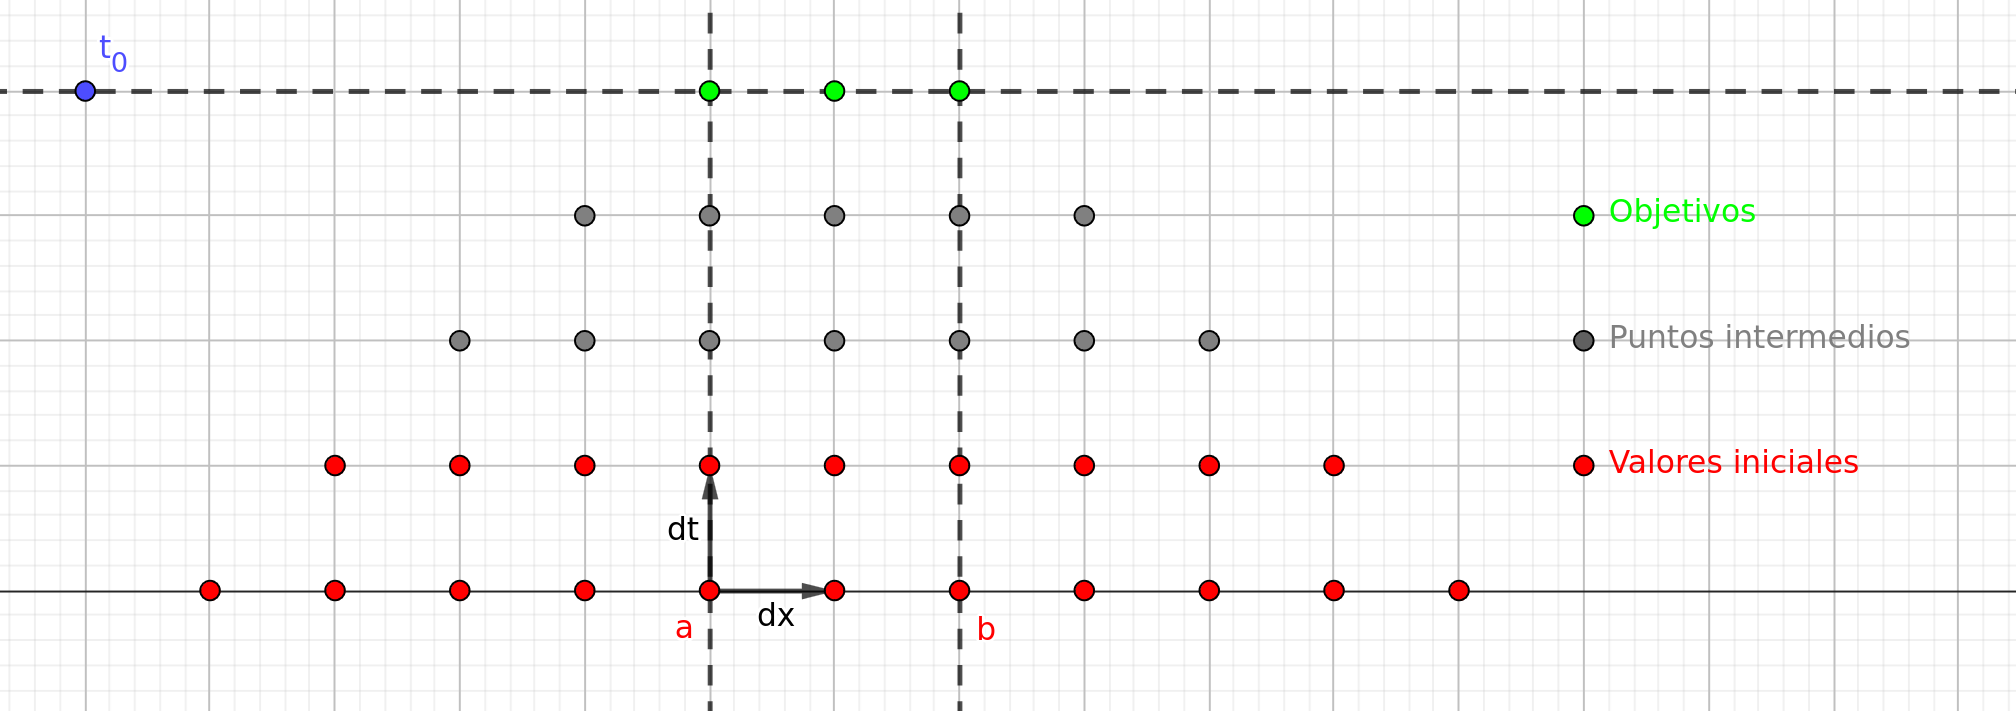
\includegraphics[width=\linewidth]{./Imagenes/Bitmap/1dwavepoints.png}
	\caption{Representación en la malla del esquema \eqref{eq:1dwave_formula}}
	\label{fig:1dwave_points}
\end{figure}

Salta a la vista que, a diferencia de el caso de la ecuación del calor, vamos a necesitar calcular $U_{i,j}$ para puntos que estén fuera del intervalo objetivo, pero esto no es ningún problema, porque ya comentamos que $U_{i,j}$ está definido para cualquier $i\in\mathbb{R}$.

La convergencia del esquema numérico depende exclusivamente del valor de $\lambda$. Si $\lambda > 1$, el método diverge 
\footnote{Esto no lo probaremos, pero puede encontrarse una demostración en \cite[ p. 487.]{anummeth}}. Por otro lado, si $\lambda <=1$, el esquema converge.

\begin{teorema}
	Si $\lambda=1$ y $f,g$ son dos funciones continuas con derivada continua, la aproximación dada por \eqref{eq:1dwave_formula} converge a la solución de \eqref{eq:1dwave} cuando $\Delta x = c\Delta t \longrightarrow 0$.
\end{teorema}
\begin{proof}
	Primero definimos el siguiente valor.
	\begin{equation}
		D_{i,j} := U_{i,j} - U_{i-1,j-1} \hspace{20px} \forall 1<=j.
	\end{equation}
	Como $\lambda = 1$ podemos rescribir la ecuación \eqref{eq:1dwave_formula} como 
	\begin{equation}
		U_{i,j+1} - U_{i-1,j} = U_{i+1,j} - U_{i,j-1} \Rightarrow D_{i,j+1} = D_{i+1,j}.
	\end{equation}
	Aplicando ahora esa fórmula de manera recursiva, podemos observar la siguiente relación
	\begin{equation}
		\label{aux}
		D_{i,j+1} = D_{i+k,j-k+1} \hspace{20px} \forall 0<=k<=j.
	\end{equation}
	Además, por como ha sido definido $D$, es fácil observar que para cualquier $j\geq1$, se tiene que
	\begin{equation}
		\sum_{k=0}^{j}D_{i-k,j-k+1} = U_{i,j+1} - U_{i-j,0},
	\end{equation}
	de donde podemos despejar la fórmula explícita
	\begin{equation}
		U_{i,j+1} = U_{i-j-1,0} + \sum_{k=0}^{j}D_{i-k,j-k+1}.
	\end{equation}
	Si tenemos en cuenta que $u_{i-j-1,0}=f_{i-j-1}$, y gracias a \eqref{aux}, podemos sustituir los sumandos del sumatorio por términos más simples, y obtener
	\begin{equation}
		U_{i,j+1} = f_{i-j-1} + \sum_{k=0}^{j}D_{i+j-2k,1} = f_{i-j-1} + \sum_{k=0}^{j}(U_{i+j-2k,1} - U_{i+j-2k-1,0}).
	\end{equation}
	El valor exacto de $U_{i,0}$ y $U_{i,1}$ es $f_{i}$ y $f_i+\Delta tg_i$ respectivamente, por lo que podemos sustituir y obtener
	\begin{equation}
		\label{aux2}
		U_{i,j+1} = f_{i-j-1} + \Delta t\sum_{k=0}^{j}g_{i+j-2k} + \sum_{k=0}^{j}(f_{i+j-2k}-f_{i+j-2k-1}).
	\end{equation}
	
	Esto es una representación exacta (y no recursiva) del valor de $U_{i,j+1}$. Vamos a demostrar que ese valor tiende a $u_{i,j+1}$ cuando hacemos la malla más pequeña.
	Como $t_n=n\Delta t$, se tiene que $x_n=n\Delta x=nc\Delta t=ct_{n}$, por ello, para cualquier función $F$ se tiene que $F_{i+j}:=F(x_{i+j})=F(x_i+ct_j)$.
	
	Como $f$ tiene derivada continua, usando el teorema del valor medio obtenemos que $\exists\theta_k\in(-1,0)$ tal que
	\begin{equation}
		f_{i+j-2k}-f_{i+j-2k-1} = f(x_{i-2k}+ct_j) - f(x_{i-2k}+ct_{j}-\Delta x) = \Delta xf'(x_{i-2k}+ct_j+\theta_k\Delta x).
	\end{equation} 

	Además, $f_{i-j-1}=f(x_{i-j-1})=f(x_i-(j+1)\Delta x)=f(x_i -(j+1)c\Delta t)=f(x_i-ct_{j+1})$. Haciendo algo muy similar, obtenemos las igualdades $g_{i+j-2k}=g(x_i+ct_{j+1}-[2k+1]\Delta x)$ y $f'(x_{i-2k}+ct_j+\theta_k\Delta x)=f'(x_i+ct_{j+1}+\theta_k\Delta x - [2k+1]\Delta x)$.
	
	Sean $x$,$t$ puntos de la malla, hagamos tender $\Delta x=c\Delta t$ a 0. Como son puntos de la malla, tienen que existir $i$ y $j$ (dependientes de $\Delta x$ y $\Delta t$ y que tienden a infinito cuando estos tienden a cero) tales que $x=x_i$ y $t=t_j$.
	Si sustituimos en \eqref{aux2} con todas las igualdades que hemos obtenido, tendremos
	\begin{multline}
		U_{i,j+1} = f(x_i-ct_{j+1}) + \frac{1}{2c}\sum_{k=0}^{j}2\Delta xg(x_i+ct_{j+1}-[2k+1]\Delta x) + \\ \frac{1}{2}\sum_{k=0}^{j}2\Delta xf'(x_i+ct_{j+1} +\theta_k\Delta x - [2k+1]\Delta x).
	\end{multline}
	
	Observemos con detenimiento el primer sumatorio, cada sumando es la función $g(x_i+ct_j - \xi)$ multiplicada por $2\Delta x$ y evaluada en el punto $\xi_k\in \{\Delta x, 3\Delta x,\dots, (2j+1)\Delta x\}$, cada uno de estos puntos pertenece al intervalo $[(2k)\Delta x, (ki+2)\Delta x]$, que tiene tamaño $2\Delta x$. Salta a la vista que hemos creado una partición del intervalo $[0,(2j+2)\Delta x] = [0,2ct_{j+1}]$. Utilizando la definición de integral, se tiene que el primer sumatorio es la integral
	\begin{equation}
		\frac{1}{2c}\sum_{k=0}^{j}2\Delta xg(x_i+ct_{j+1}-[2k+1]\Delta x) = \frac{1}{2c}\int_{0}^{2ct_{j+1}}g(x_i+ct_{j+1}-\xi)d\xi,
	\end{equation}
	y, de manera completamente análoga, llegamos a que el segundo sumando también se puede expresar como la siguiente integral
	\begin{equation}
		\frac{1}{2}\sum_{k=0}^{j}2\Delta xf'(x_i+ct_{j+1} +\theta_k\Delta x - [2k+1]\Delta x) = \frac{1}{2}\int_{0}^{2ct_{j+1}} f'(x_i+ct_{j+1}-\xi)d\xi.
	\end{equation}
	
	Teniendo en cuenta las igualdades que acabamos de ver (y  que $x=x_i$ y $t=t_j+1$), podemos ver que al pasar al límite, la fórmula se nos queda como
	\begin{equation}
		U(x,t) = f(x-ct) + \frac{1}{2c}\int_{0}^{2ct}g(x+ct-\xi)d\xi + \frac{1}{2}\int_{0}^{2ct} f'(x+ct-\xi)d\xi.
	\end{equation}

	Si realizamos el cambio de variable $\nu = x +ct - \xi$ sobre la primera integral, se nos queda en
	\begin{equation}
		\int_{x-ct}^{x+ct}g(\mu)d\mu.
	\end{equation}
	Además es fácil comprobar que la función $-f(x+ct-\xi)$ es una primitiva de $f'(x+ct-\xi)$ (si la consideramos una función en la variable $\xi$), por lo que, aplicando el segundo teorema fundamental del cálculo, tenemos que la segunda integral vale
	\begin{equation}
		\frac{1}{2}[-f(x+ct-2ct)+f(x+ct)] = \frac{1}{2}[f(x+ct)-f(x-ct)].
	\end{equation}
	
	Por último, si sustituimos las integrales originales por la integral y el valor que acabamos de calcular, concluimos que
	\begin{equation}
		U(x,t) = \frac{1}{2}[f(x+ct) - f(x-ct)] + \int_{x-ct}^{x+ct}g(\mu)d\mu,
	\end{equation}
	que, como calculamos en la Sección anterior, es la solución exacta del problema. Hemos probado que $\forall j\geq1$ la aproximación converge a la solución cuando hacemos más pequeñas las mallas, y sabemos que la aproximación es exacta en los valores $U_{i,0}$, por lo que hemos concluido la demostración.
	Que, pasando al límite se nos queda en
\end{proof}

	Este teorema demuestra que si $\lambda=1$ el método converge a la solución, pero como veremos es realmente útil poder utilizar $\lambda<1$ de cara a hacer algoritmos que se aprovechen del paralelismo en la CPU, por lo que enunciaremos el siguiente resultado, cuya demostración puede encontrarse en \cite{anummeth}.
	
	\begin{teorema}
		Si $\lambda\leq1$ y $f,g$ son dos funciones continuas con derivada continua, la aproximación dada por \eqref{eq:1dwave_formula} converge a la solución de \eqref{eq:1dwave} cuando $\Delta x = c\Delta t \longrightarrow 0$.
	\end{teorema}

\section{Caso bidimensional}


